\setcounter{page}{2}
\begin{center}
    \textbf{ПРОТОКОЛ}
\end{center}
\begin{figure}[H]
    \centering
    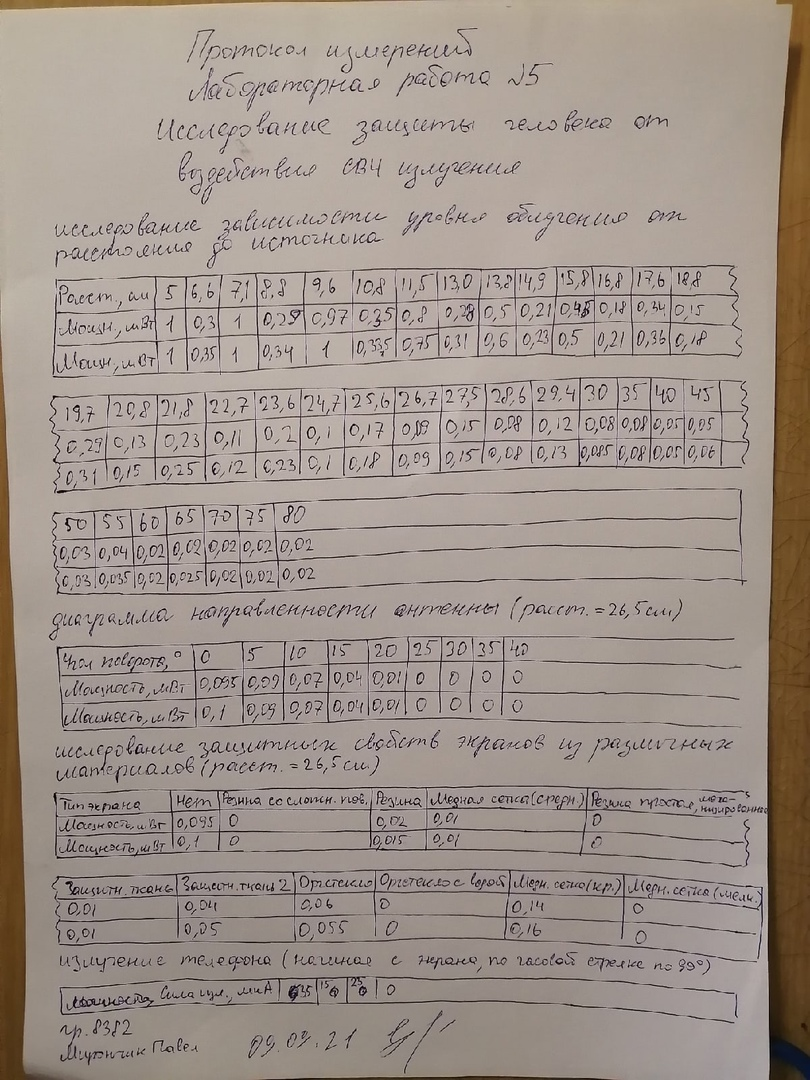
\includegraphics[width=16cm]{protocol}
    \label{fig:protocol}
\end{figure}
\pagebreak
\section*{Исследование зависимости уровня облучения от расстояния до источника.}

Для каждого уровня расстояния значение мощности было измерено дважды, первая строка
содержит последовательность значений, полученных удалением приемника от генератора, а вторая --
при движении приемника обратно в направлении к генератору.
Для практического расчета значений плотности потока энергии воспользуемся формулами ниже
\begin{displaymath}
    \text{ППЭ}_\text{э} = \frac{P_{\text{пр}}}{S_{\text{эф}}}
\end{displaymath}
где $P_{\text{пр}}$ -- измеренное значение мощности, $S_{\text{эф}}$ -- эффективная площадь
приемной антенны, которую можно вычислить по формуле
\begin{displaymath}
    S_{\text{эф}} = \frac{\lambda^2}{4\pi} G_{\text{пр}}
\end{displaymath}

В данной работе коэффициент усиления приёмной и передающей антенн $G_{\text{п}} = G_{\text{пр}} = 55$.
Длина волны СВЧ-излучения в воздухе $\lambda = 3 \text{см}$.

Рассчитаем значение плотность потока энергии для каждого измеренного значения длины (см. табл. 1).

\vspace{0.4cm}
\noindent\textit{Таблица 1 -- Плотность потока энергии от расстояния}

\begin{longtable}{|p{3cm}|p{3cm}|p{3cm}|p{3cm}|p{3cm}|}
    \hline
    $l$, см. & $P_{\text{пр1}}$, мВт & $P_{\text{пр2}}$, мВт & $\text{ППЭ}_{\text{э1}}$, $\frac{\text{Вт}}{\text{м}^2}$ & $\text{ППЭ}_{\text{э2}}$, $\frac{\text{Вт}}{\text{м}^2}$ \\\hline
    5.0      & 1.00                  & 1.000                 & 0.253866                                                 & 0.253866                                                 \\\hline
    6.6      & 0.30                  & 0.350                 & 0.076160                                                 & 0.088853                                                 \\\hline
    7.1      & 1.00                  & 1.000                 & 0.253866                                                 & 0.253866                                                 \\\hline
    8.8      & 0.29                  & 0.340                 & 0.073621                                                 & 0.086314                                                 \\\hline
    9.6      & 0.97                  & 1.000                 & 0.246250                                                 & 0.253866                                                 \\\hline
    10.8     & 0.35                  & 0.335                 & 0.088853                                                 & 0.085045                                                 \\\hline
    11.5     & 0.80                  & 0.750                 & 0.203093                                                 & 0.190400                                                 \\\hline
    13.0     & 0.28                  & 0.310                 & 0.071083                                                 & 0.078698                                                 \\\hline
    13.8     & 0.50                  & 0.600                 & 0.126933                                                 & 0.152320                                                 \\\hline
    14.9     & 0.21                  & 0.230                 & 0.053312                                                 & 0.058389                                                 \\\hline
    15.8     & 0.45                  & 0.500                 & 0.114240                                                 & 0.126933                                                 \\\hline
    16.8     & 0.18                  & 0.210                 & 0.045696                                                 & 0.053312                                                 \\\hline
    17.6     & 0.34                  & 0.360                 & 0.086314                                                 & 0.091392                                                 \\\hline
    18.8     & 0.15                  & 0.180                 & 0.038080                                                 & 0.045696                                                 \\\hline
    19.7     & 0.29                  & 0.310                 & 0.073621                                                 & 0.078698                                                 \\\hline
    20.8     & 0.13                  & 0.150                 & 0.033003                                                 & 0.038080                                                 \\\hline
    21.8     & 0.23                  & 0.250                 & 0.058389                                                 & 0.063467                                                 \\\hline
    22.7     & 0.11                  & 0.120                 & 0.027925                                                 & 0.030464                                                 \\\hline
    23.6     & 0.20                  & 0.230                 & 0.050773                                                 & 0.058389                                                 \\\hline
    24.7     & 0.10                  & 0.100                 & 0.025387                                                 & 0.025387                                                 \\\hline
    25.6     & 0.17                  & 0.180                 & 0.043157                                                 & 0.045696                                                 \\\hline
    26.7     & 0.09                  & 0.090                 & 0.022848                                                 & 0.022848                                                 \\\hline
    27.5     & 0.15                  & 0.150                 & 0.038080                                                 & 0.038080                                                 \\\hline
    28.6     & 0.08                  & 0.080                 & 0.020309                                                 & 0.020309                                                 \\\hline
    29.4     & 0.12                  & 0.130                 & 0.030464                                                 & 0.033003                                                 \\\hline
    30.0     & 0.08                  & 0.085                 & 0.020309                                                 & 0.021579                                                 \\\hline
    35.0     & 0.08                  & 0.080                 & 0.020309                                                 & 0.020309                                                 \\\hline
    40.0     & 0.05                  & 0.050                 & 0.012693                                                 & 0.012693                                                 \\\hline
    45.0     & 0.05                  & 0.060                 & 0.012693                                                 & 0.015232                                                 \\\hline
    50.0     & 0.03                  & 0.030                 & 0.007616                                                 & 0.007616                                                 \\\hline
    55.0     & 0.04                  & 0.035                 & 0.010155                                                 & 0.008885                                                 \\\hline
    60.0     & 0.02                  & 0.020                 & 0.005077                                                 & 0.005077                                                 \\\hline
    65.0     & 0.02                  & 0.025                 & 0.005077                                                 & 0.006347                                                 \\\hline
    70.0     & 0.02                  & 0.020                 & 0.005077                                                 & 0.005077                                                 \\\hline
    75.0     & 0.02                  & 0.020                 & 0.005077                                                 & 0.005077                                                 \\\hline
    80.0     & 0.02                  & 0.020                 & 0.005077                                                 & 0.005077                                                 \\\hline
\end{longtable}

Усредним полученные экспериментально значения плотности потока энергии и отобразим
на графике зависимость от расстояния (см. рис. 1).

\begin{figure}[H]
    \centering
    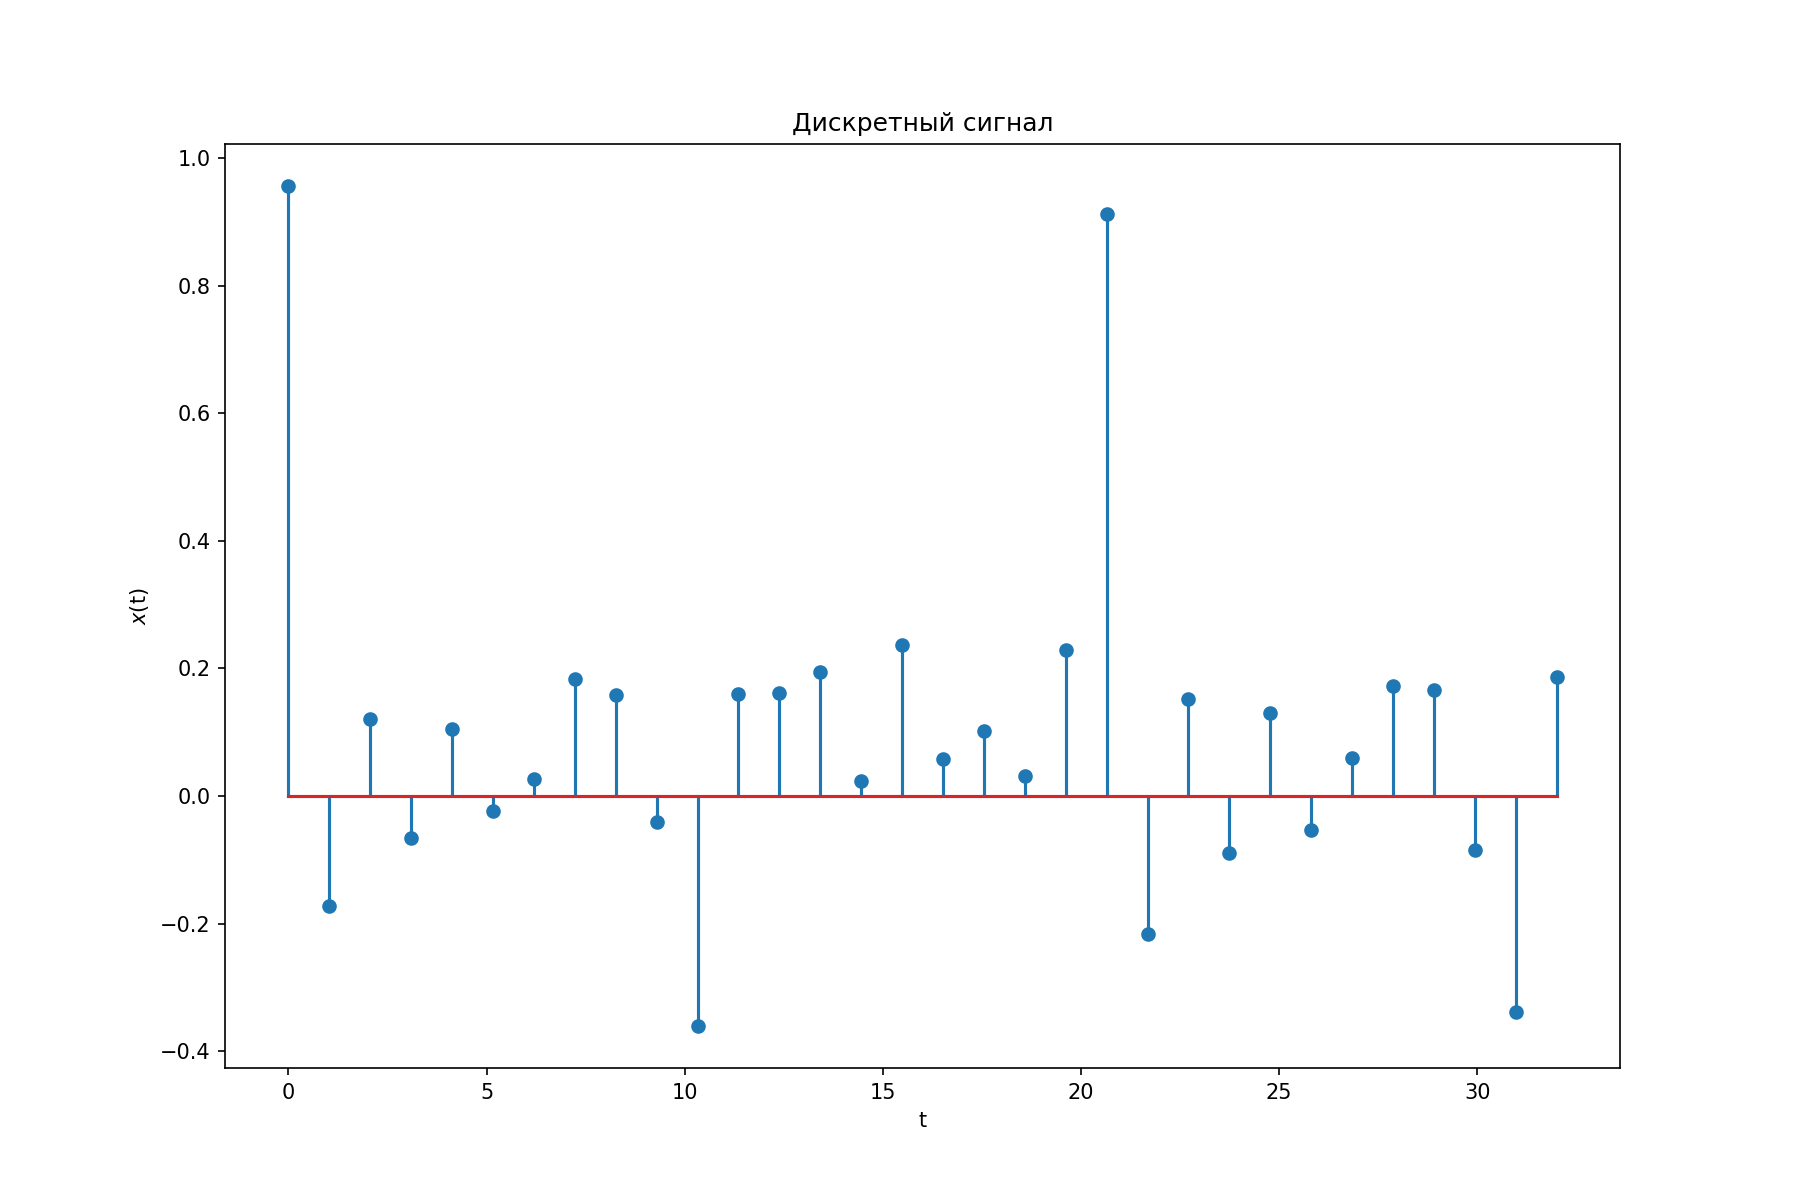
\includegraphics[width=14cm]{1}
    \caption*{Рисунок 1 -- Экспериментальная зависимость ППЭ от расстояния}
    \label{fig:1}
\end{figure}

Пространство около излучающей антенны условно делится на ближнюю, переходную и дальнюю зоны
В данной работе границы равны 9 и 27 см соответственно.
Теоретический вид зависимости представлен на рисунке 2.

\begin{figure}[H]
    \centering
    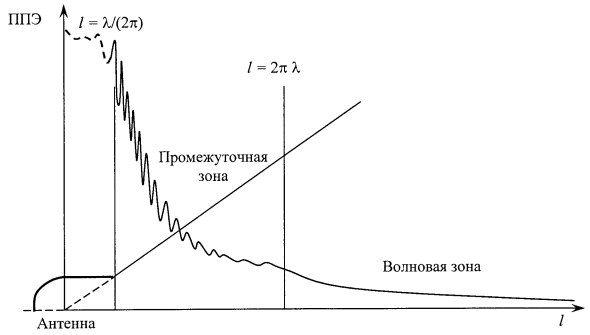
\includegraphics[width=14cm]{2}
    \caption*{Рисунок 2 -- Теоретический вид зависимости ППЭ от расстояния}
    \label{fig:2}
\end{figure}

В промежуточной зоне наблюдается сложный характер зависимости напряженностей
электромагнитного и магнитного полей от расстояния.
На рисунке 1 при значении расстояния до примерно 30 см график рваный, сильно осциллирующий.
При переходе в дальнюю зону график становится более гладким.

В целом, характер полученной экспериментальным методом зависимости совпадает
с теоретической (рисунки 1 и 2).

Проведем расчет плотности потока энергии для собранных данных с использованием
теоретической формулы
\begin{displaymath}
    \text{ППЭ}_\text{т} = \frac{P_{\text{г}} G_{\text{п}}}{4\pi l^2} F^2
\end{displaymath}
где $P_{\text{г}} = 4 \text{мВт}$ -- выходная мощность генератора, $F$ -- коэффициент
искажения.
В первом приближении примем $F$ равным 1.

Проведем расчет для $l$ от 30 см, т.е. в дальней зоне.
Результат приведен в таблице 2.

\pagebreak
\noindent\textit{Таблица 2 -- Теоретическая плотность потока энергии от расстояния для дальней зоны}

\begin{longtable}{|p{7.5cm}|p{7.5cm}|}
    \hline
    $l$, см. & $\text{ППЭ}_{\text{т}}$, $\frac{\text{Вт}}{\text{м}^2}$ \\\hline
    30.0     & 0.194523                                                \\\hline
    35.0     & 0.142915                                                \\\hline
    40.0     & 0.109419                                                \\\hline
    45.0     & 0.086455                                                \\\hline
    50.0     & 0.070028                                                \\\hline
    55.0     & 0.057875                                                \\\hline
    60.0     & 0.048631                                                \\\hline
    65.0     & 0.041437                                                \\\hline
    70.0     & 0.035729                                                \\\hline
    75.0     & 0.031124                                                \\\hline
    80.0     & 0.027355                                                \\\hline
\end{longtable}

График зависимости $\text{ППЭ}_{\text{т}}$ от расстояния приведен на рисунке 3.
\begin{figure}[H]
    \centering
    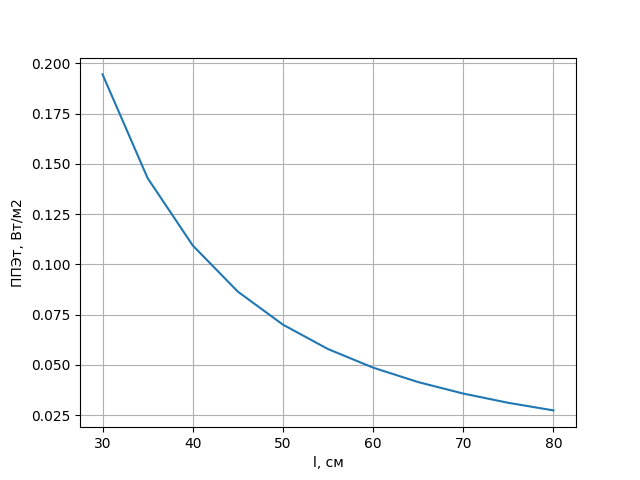
\includegraphics[width=14cm]{3}
    \caption*{Рисунок 3 -- Теоретическая зависимость ППЭ от расстояния}
    \label{fig:3}
\end{figure}

Теоретические значения расходятся со значениями, полученными экспериментально, примерно
на 1 порядок.
Это может быть связано с выбором коэффициента искажения и коэффициента усиления
передающей и приемной антенн, которые были выбраны константными, но
на самом деле, могут иметь более сложную зависимость от расстояния.

\section*{Снятие диаграммы направленности.}
Приемник был закреплен на расстоянии 26.5 см.

Зависимость мощности от угла поворота представлена на рисунке 4.
В качестве мощности выбрано среднее из двух измерений для соответствующего угла.

\begin{figure}[H]
    \centering
    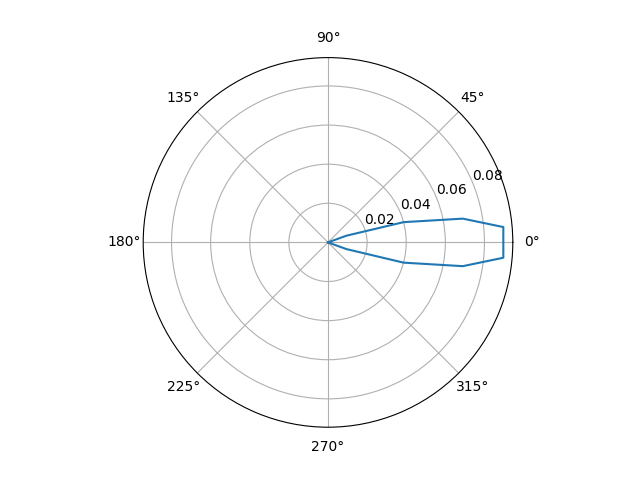
\includegraphics[width=14cm]{4}
    \caption*{Рисунок 4 -- Диаграмма направленности антенны}
    \label{fig:4}
\end{figure}

Заметим, что при выборе угла в 25 градусов, мощность равна нулю.
Так как генератор однонаправленный, то для избежания воздействия изучения
достаточно отойти от источника на угол, превышающий 25 градусов.

\section*{Исследование защитных свойств экранов из различных материалов.}
Приемник был закреплен на расстоянии 26.5 см.

Вычислим среднее арифметическое измеренных мощностей, коэффициент ослабления/экранирования
излучения разными экранами по формуле
\begin{displaymath}
    K_{\text{экр}} = \frac{P_\text{б.экр.}}{P_\text{экр.}}
\end{displaymath}
где $P_\text{б.экр.}$ -- измеренная мощность излучения без экрана, $P_\text{экр.}$ -- мощность
излучения с экраном.

Результаты вычислений приведены в таблице 3.

\noindent\textit{Таблица 3 -- Защитные свойства экранов из различных материалов}
\begin{longtable}{|p{5cm}|p{2.5cm}|p{2.5cm}|p{2.5cm}|p{2.5cm}|}
    \hline
    Тип экрана                   & $P_\text{пр1}$, мВт & $P_\text{пр2}$, мВт & $P_\text{ср.}$, мВт & $K_{\text{экр}}$ \\\hline
    Без экрана                   & 0.095               & 0.100               & 0.0975              & 1.000000         \\\hline
    Резина (сложная поверхность) & 0.000               & 0.000               & 0.0000              & $\to \infty$     \\\hline
    Резина                       & 0.020               & 0.015               & 0.0175              & 5.571429         \\\hline
    Медная сетка (средн.)        & 0.010               & 0.010               & 0.0100              & 9.750000         \\\hline
    Резина механизированная      & 0.000               & 0.000               & 0.0000              & $\to \infty$     \\\hline
    Защитная ткань 1             & 0.010               & 0.010               & 0.0100              & 9.750000         \\\hline
    Защитная ткань 2             & 0.040               & 0.050               & 0.0450              & 2.166667         \\\hline
    Оргстекло                    & 0.060               & 0.055               & 0.0575              & 1.695652         \\\hline
    Оргстекло с водой            & 0.000               & 0.000               & 0.0000              & $\to \infty$     \\\hline
    Медная сетка (кр.)           & 0.140               & 0.160               & 0.1500              & 0.650000         \\\hline
    Медкая сетка (мелк.)         & 0.000               & 0.000               & 0.0000              & $\to \infty$     \\\hline
\end{longtable}

Механизированная резина, резина со сложной поверхностью, оргстекло с водой и мелкая медная сетка экранируют
излучение в рассмотренном опыте.
Хуже с задачей справляются медная сетка средней мелкости и защитная ткань 1, уменьшая мощность излучения на 1 порядок.
Остальные материалы не рекомендуются в качестве экранов в силу малого
коэффициента экранирования.

\section*{Расчет безопасного расстояния до антенны без экрана.}
Проведем расчет безопасного расстояния для заданной антенны мощностью 4 мВт без экрана.
Расчет будем проводить для кратковременно облучения.
В этом случае максимальное значение $\text{ЭЭ}_{\text{ППЭ}_\text{ПД}}$ не должно
превышать $10 \text{мкВт} / \text{см}^2 = 0.1 \text{Вт} / \text{м}^2$ для постоянного и 
$10 \text{Вт} / \text{м}^2$ для кратковременного излучений.

\begin{displaymath}
    \text{ППЭ}_\text{т} = \frac{P_{\text{г}} G_{\text{п}}}{4\pi l^2} F^2
\end{displaymath}

Из этой формулы определим минимально допустимое расстояние, на котором можно находиться 
относительно источника излучения. Для постоянного такое расстояние составит $41 \text{см}$, 
для кратковременного - $4 \text{см}$.

Рекомендуется находиться в дальней зоне излучения (дальше 41 см от источника),
для исследуемой антенны уровень энергетической нагрузки не будет превышать
пределов для кратковременного облучения.


\section*{Исследование силы излучения мобильного телефона при звонке на него.}
Проанализируем излучение телефона.

Для начала определим, что антенна устройства либо ненаправленная, либо имеет очень широкий радиус излучения.
Это следует из того, что устройство излучает достаточно сильный сигнал по трем направлениям - со стороны 
экрана, правой и задней сторон 35 мкА, 15 мкА и 25 мкА соответственно. Вероятно, антенна не направленная, а
отсутствие излучения с левой стороны устройства объясняется экранированием антенны корпусом устройства.

Далее исследуем силу излучения. Выберем максимально зафиксированное значение излучения в 35 мкА. Этому 
значению соответствует ППЭ, примерно равное $11.5 \text{мкВт} / \text{см}^2$. Максимально 
допустимое значение составляет $10 \text{мкВт} / \text{см}^2$, поэтому можно было бы сказать, 
что устройство не соответствует требованиям. Тем не менее стоит учитывать, во-первых, погрешность измерений
вследствие несовершенства измерительного устройства, а во-вторых кратковременность излучения: оно возникает 
только при активном звонке с устройства при условии, что устройство воспринимает (и, соответственно, передает)
какой-либо звук. Если пользователь устройства будет молчать, то излучение станет невозможно зарегистрировать
измерительным прибором, использовавшимся в этой лабораторной работе, что было также проверено, пусть и не 
отражено в протоколе измерений.